\documentclass[11pt,a4paper]{article}

\usepackage{datetime}
\usepackage{graphicx}

\title{Chapter 4: Communication}
\newdate{date}{11}{05}{2020}
\date{\displaydate{date}}
\author{Nguyen Ngoc Lam - 20162316}

\begin{document}
	\pagenumbering{gobble}
  	\maketitle
  	\newpage
  	\pagenumbering{arabic}
  	\tableofcontents
  	\newpage
  	
  	\section{Why in many layered protocols, each layer has its own header}
  	\begin{itemize}
  		\item Each layer must be independent of the other ones.
  		\item The data passed from the upper layer down to the lower layer contains both header and data, but the lower layer cannot tell which is which.
  		\item Having a single big header that all the layers could read
and write would make changes in the protocol of one layer visible to other layers, thus making the whole protocals unsafe.
  	\end{itemize}
  	
  	\section{Socket representation; Socket connection representation? Why do we need 4 values to represent a socket connection?}
  	A Socket is represented by:
  	\begin{itemize}
  		\item address
  		\item port
  	\end{itemize}
  	A Socket Connection is represented by;
  	\begin{itemize}
  		\item local-address
  		\item local-port
  		\item foreign-address
  		\item foregin-port
  	\end{itemize}
  	Why do we need 4 values to represented a socket connection:
  	\begin{itemize}
  		\item Each socket has 2 fields: address and port
  		\item A Socket Connection is defined by 2 sockets: local and foreign
  		\item To represent a Connection, we need to represent that 2 sockets
  	\end{itemize}
  	
  	\section{Three characteristics of TCP protocol}
  	\begin{itemize}
  		\item \textbf{\emph{Connection-Oriented}}: TCP requires that devices first establish a connection with each other before they send data. The connection creates the equivalent of a circuit between the units, and is analogous to a telephone call. A process of negotiation occurs to establish the connection, ensuring that both devices agree on how data is to be exchanged.
  		\item \textbf{\emph{Reliable}}: Communication using TCP is said to be \emph{reliable} because TCP keeps track of data that has been sent and received to ensure it all gets to its destination. As we saw in the previous topic, TCP can't really “guarantee” that data will always be received. However, it \emph{can} guarantee that all data sent will be checked for reception, and checked for data integrity, and then retransmitted when needed. So, while IP uses “best effort” transmissions, you could say TCP \emph{tries harder}, as the old rent-a-car commercial goes.
  		\item \textbf{\emph{Synchronous}}: All transmissions in TCP are \emph{acknowledged} (at the TCP layer—TCP cannot guarantee that all such transmissions are received by the remote application). The recipient must tell the sender \emph{“yes, I got that”} for each piece of data transferred, which is different from typical messaging protocols where the sender never knows what happened to its transmission
  	\end{itemize}
  	On UDP, they are:
  	\begin{itemize}
  		\item Conection-less
  		\item Unreliable: since it did not provide acknowledgement messages, it can not check whether the messages are received
  		\item Does not provide acknowledgement messages
  	\end{itemize}
  	
  	\section{Two main issues of RPC}
  	Issues:
  	\begin{itemize}
  		\item \textbf{\emph{Marshalling}}:Parameters must be marshalled into a standard representation.
  		\item \textbf{\emph{Binding}}: How does the client know who to call, and where the service resides?
  	\end{itemize}
  	
  	\section{Consider a procedure incr with two integer parameters. The procedure adds ONE to each parameter. Now suppose that it is called with the same variable twice, for example, as incr(i, i). If i is initially 0, what value will it have afterward if call-by-reference is used? How about if copy/restore is used?}
  	If call by reference is used, a pointer to $ i $ is passed to $incr$. It will be incremented two times, so the final result will be two. However, with copy/restore,$ i $ will be passed by value twice, each value initially 0. Both will be incremented, so both will now be 1. Now both will be copied back, with the second copy overwriting the first one. The final value will be 1, not 2.
  	
  	\section{Explain why transient synchronous communication has inherent scalability problems, and how these could be solved}
  	Problems:
  	\begin{itemize}
  		\item Scalability is the ability for a distributed application to expand without affecting any of the application algorithms.
  		\item The transient synchronous communication would have issues pertaining to geographical scalability. If the client and the server are placed in two far-away geographical locations it would take a considerable amount of time for the client to send a request and receive a reply.
  		\item Because the client remains idle until it receives the reply there is a considerable waste of time, since the client can only resume after receiving the reply. If the system is always in idle mode all of the time as it is synchronous there would not be any room for scalability.
  		\item This issue is a performance issue which creates unnecessary network latency.
  		\item There is set back when it comes to expanding of the system because it is transient system there is no storage. If there was to be a malfunction or failure of one component the whole system would be down. This is because the system is not persistent.
  	\end{itemize}
	Solutions:
	\begin{itemize}
		\item We can use network optimization tools. These tools help to minimize the amount traffic being built up on the network.
		\item Another solution would be to change to a new upgraded network connection. A faster network connection is key factor to reduce the time taken to receive a reply for request sent to the server from the client.
	\end{itemize}

	\section{Can we apply the persistent asynchronous communication to RPC? Explain it}
	Yes, but only on a hop-to-hop basis in which a process managing a queue
passes a message to a next queue manager by means of an RPC.\\
	Effectively, the service offered by a queue manager to another is the storage of a message. The calling queue manager is offered a proxy implementation of the interface to the remote queue, possibly receiving a status indicating the success or failure of each operation. In this way, even queue managers see only queues and no further communication.
	
	\section{In message-oriented transient communication, why the client doesn’t need to call the bind primitive to bind its socket to a port?}
	Because the operating systemcan dynamically allocate a port when the connection is set up.
	
	\section{In message-oriented transient communication, explain the role of the two queues (completed and incomplete connection queue) maintained by TCP for a listening socket. Explain the backlog parameter of the function listen called by a TCP server.}
	Role of the two queues:
	\begin{itemize}
		\item  Transient communication means the way by which the messages are not saved into a buffer to wait for its delivery at the message receiver, which means the messages will be delivered only if both the systems (sender and receiver) are running.
		\item The role of completed connections queue: store the connections that are ready to send message.
		\item  The role of incompleted connections queue: store the connections that are not ready to send message.
		\item Together, they will prevent sending messages over when the receiver is not ready thus making the messages lost in the process 
	\end{itemize}
	Role of \emph{backlog} parameter of the function \emph{listen} called by a TCP server
	\begin{itemize}
		\item The backlog argument specifies the maximum number of queued connections and should be at least 0; the maximum value is system-dependent (usually 5), the minimum value is forced to 0.
		\item In simple words, the backlog parameter specifies the number of pending connections the queue will hold.
	\end{itemize}
	
	\section{What is the role of Message-Queuing System in persistent communication?}
	Roles:
	\begin{itemize}
		\item Offer the intermediate-term storage capacity for messages
		\item Target to support message transfers that are allowed to takeminutes insteadof seconds or milliseconds
		\item No guarantees about when or even if the message will be actually read
		\item Allow the sender and receiver can execute completely independently
	\end{itemize}
	
	\section{Bit-rate, Delay and Jitter}
	\begin{enumerate}
		\item Bit-rate
			\begin{itemize}
				\item The number of bits that are conveyed or processed per unit of time
				\item Used to determine the bandwidth (the maximum rate that information can be transferred
				\item Higher bit-rate means better bandwidth thus could led to better quality of the content transfer through the channel
			\end{itemize}
		\item Delay
			\begin{itemize}
				\item Also called Lantency, is defined as the delay between the sender and the receiver decoding it
				\item Mainly a function of the signals travel time, and processing time at any nodes the information traverses
				\item Lower delay means better service. High latency can render an application with high prioriy on synchonization such as VoIP or online gaming unusable.
			\end{itemize}
		\item Jitter
			\begin{itemize}
				\item Variation in packet delay at the receiver of the information.
				\item Can be quantified in the same terms as all time-varying signals
				\item High jitter may cause a display monitor to flicker, affect the performance of processors in personal computers, introduce clicks or other undesired effects in audio signals, and cause loss of transmitted data between network devices
			\end{itemize}
	\end{enumerate}
	
	\section{How we can use a buffer at the receiver to reduce the jitter}
	\begin{itemize}
		\item Jitter buffers eliminate jitter by queuing a number of packets to absorb the delay differences between them and then playing them out at a constant rate
		\item This gives the more delayed packets a chance to catch up so that all packets are output smoothly
		\item As with any type of buffering, the larger the jitter buffer is, the longer a packet's playout delay becomes
	\end{itemize}
	\begin{figure}[h!]
  		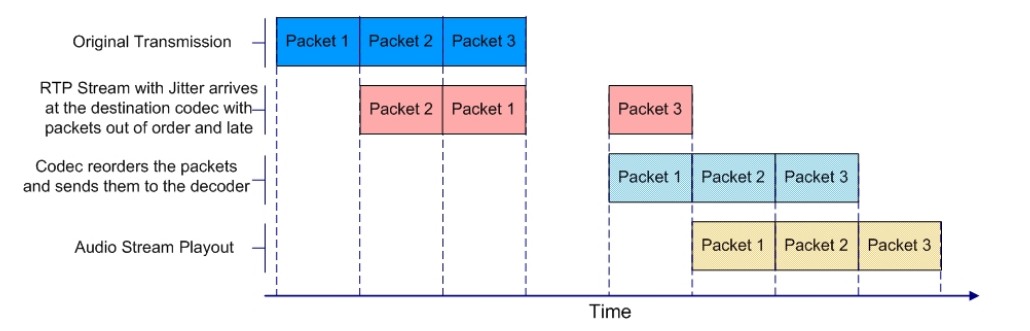
\includegraphics[width=\linewidth]{buf-vis.png}
  		\caption{Visualization of how the buffer works}
  		\label{fig:bufvis}
	\end{figure}
	
	\section{Forward error correction (FEC)}
	\begin{itemize}
		\item Forward error correction (FEC) is an error correction technique to detect and correct a limited number of errors in transmitted data without the need for retransmission.
		\item The sender sends a redundant error-correcting code along with the data frame
		\item The receiver performs necessary checks based upon the additional redundant bits. If it finds that the data is free from errors, it executes error-correcting code that generates the actual frame then removes the redundant bits before passing the message to the upper layers.
		\item Error-correcting code can be broadly categorized into two types, namely, block codes and convolution codes
			\begin{itemize}
				\item \textbf{\emph{Block codes}}: The message is divided into fixed-sized blocks of bits to which redundant bits are added for error correction
				\item \textbf{\emph{Convolutional codes}}: The message comprises of data streams of arbitrary length and parity symbols are generated by the sliding application of a Boolean function to the data stream
			\end{itemize}
	\end{itemize}
\end{document}